\begin{homeworkProblem}

\textbf{Example II in the Lecture, Section 4}

(a) Implement a Metropolis-Hastings algorithm.

(b) Implement a Hamiltonian Monte Carlo algorithm

(c) Implement with the Acceptance-Rejection Method.

(d) Compare the above three algoxithms with corresponding pros and cons.

\solution

The target distribution's PDF is
$$f(x) = 0.4\cdot \dfrac{1}{\sqrt{2\pi}}e^{-\frac{1}{2}(x-2)^2} + 0.6\cdot \dfrac{1}{\sqrt{2\pi}}e^{-\frac{1}{2}(x+2)^2}, -\infty<x<\infty$$

(a) Take the $\N(0,1)$ as the proposal distribution, i.e. the one step transition PDF is
$$f_{x,y} = \dfrac{1}{\sqrt{2\pi}}e^{-\frac{1}{2}y^2}$$
So the acceptance rate is:
$$a_{x,y}=\min\left(\dfrac{\pi_yf_{y,x}}{\pi_xf_{x,y}},1\right)=\min\left(\dfrac{2e^{2y-2}+3e^{-2y-2}}{2e^{2x-2}+3e^{-2x-2}},1\right)$$
Apply the Metropolis-Hastings algorithm to generate samples as follows:
\begin{figure}[h]
    \centering
    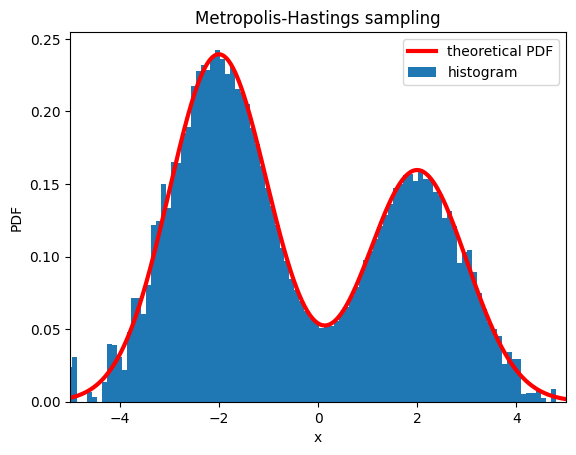
\includegraphics[width=0.5\textwidth]{./figure/p11/MH.png}
\end{figure}


(b) Since $\pi_x$ is a the stationary of the target distribution, and we can ignore the constant form, so the potential energy is
$$U(x)=-\log(\pi_x) \stackrel{\text{ignore const}}{\Rightarrow} U(x)= -\log\left(2e^{-\frac{1}{2}(x-2)^2} + 3e^{-\frac{1}{2}(x+2)^2}\right)$$
And let the mass be 1, then the Kinetic energy is
$$V(\omega)=\dfrac{1}{2}\omega^2, \quad\text{where } \omega\sim\N(0,1)$$
Thus the Hamiltonian energy is
$$H(x,\omega)=U(x)+V(\omega)= -\log\left(2e^{-\frac{1}{2}(x-2)^2} + 3e^{-\frac{1}{2}(x+2)^2}\right)+\dfrac{1}{2}\omega^2$$
Initially, set $x_0=0, \omega_0\sim\N(0,1)$, apply the Leapfrog method to sample:
\begin{align*}
\omega_{t+\frac{\delta}{2}} &= \omega_t - \frac{\delta}{2}\cdot \dfrac{\dU(x_t)}{\dx_t} = \omega_t - \frac{\delta}{2}\cdot \dfrac{2(x_t-2)e^{-\frac{1}{2}(x_t-2)^2}+3(x_t+2)e^{-\frac{1}{2}(x_t+2)^2}}{2e^{-\frac{1}{2}(x_t-2)^2}+3e^{-\frac{1}{2}(x_t+2)^2}} \\
x_{t+\delta} &= x_t + \delta \cdot \dfrac{\dV(\omega_{t+\frac{\delta}{2}})}{\domega_{t+\frac{\delta}{2}}} = x_t + \delta\cdot \omega_{t+\frac{\delta}{2}} \\
\omega_{t+\delta} &= \omega_{t+\frac{\delta}{2}} - \frac{\delta}{2}\cdot \dfrac{\dU(x_{t+\delta})}{\dx_{t+\delta}} = \omega_{t+\frac{\delta}{2}} - \frac{\delta}{2}\cdot \dfrac{2(x_{t+\delta}-2)e^{-\frac{1}{2}(x_{t+\delta}-2)^2}+3(x_{t+\delta}+2)e^{-\frac{1}{2}(x_{t+\delta}+2)^2}}{2e^{-\frac{1}{2}(x_{t+\delta}-2)^2}+3e^{-\frac{1}{2}(x_{t+\delta}+2)^2}}
\end{align*}
After Leapfrog $L$ steps, we can get the state $(x_L, \omega_L)$. And set $(x_L, -\omega_L)$ to be the proposal distribution. And the accept rate for the Hamiltonian Monte Carlo algorithm is
$$a_{(x_0,\omega_0),(x_L,-\omega_L)}=\min\left(\dfrac{\exp\left(-H(x_L,-\omega_L)\right)}{\exp\left(-H(x_0,\omega_0)\right)}, 1\right)=\min\left(\dfrac{\exp\left(-U(x_L)-V(-\omega_L)\right)}{\exp\left(-U(x_0)-V(\omega_0)\right)}, 1\right)$$
We step the stepsize to be $\delta=0.3, L=30$. One trajectory and sample results are as follows:
\begin{figure}[h]
    \centering
    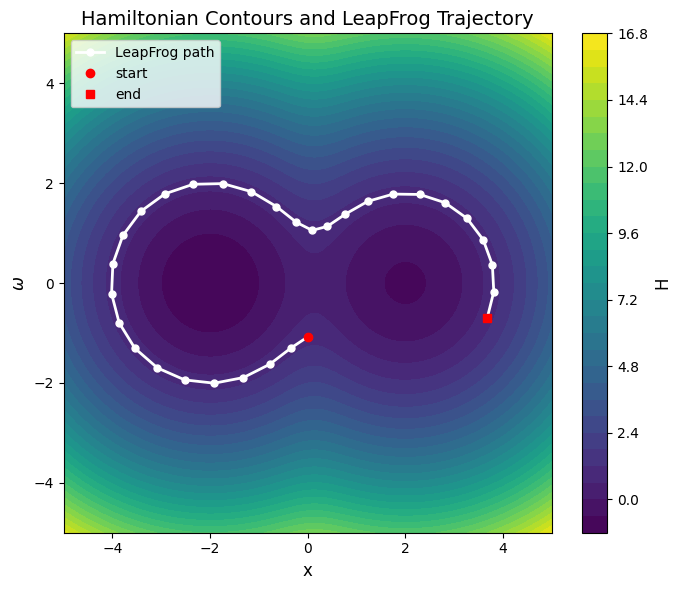
\includegraphics[width=0.5\textwidth]{./figure/p11/trajectory.png}
    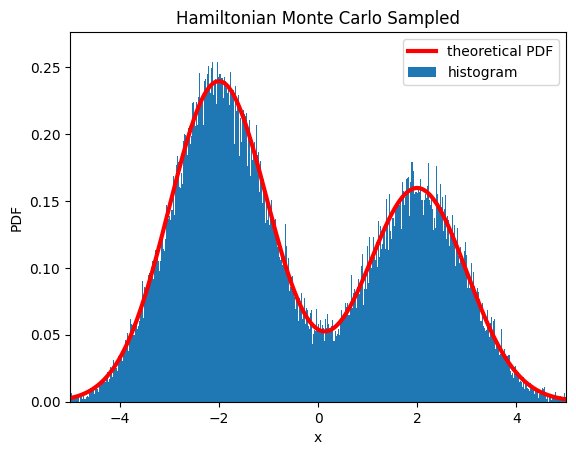
\includegraphics[width=0.5\textwidth]{./figure/p11/Hamiltonian.png}
\end{figure}

(c) We can use acceptance-rejection method to sample on $\N(0,1)$. Let $Z\sim \N(0,1)$, and $W=|Z|$. So $Z\in (-\infty,+\infty)$, $W\in (0,+\infty)$. \\
We can calculate the PDF of $W$:
$$h(x)=f_W(x)=\dfrac{2}{\sqrt{2\pi}}e^{-\frac{1}{2}x^2},x>0$$
And we can choose that $Y\sim\Expo(1)$, and its PDF is $g(y)=f_Y(y)=e^{-y},y>0$, thus we can get that
$$c = \sup_y\dfrac{h(y)}{g(y)}=\sup_y\dfrac{\frac{2}{\sqrt{2\pi}}e^{-\frac{1}{2}y^2}}{e^{-y}}=\left.\dfrac{2}{\sqrt{2\pi}}e^{-\frac{1}{2}y^2+y}\right|_{y=1}=\sqrt{\dfrac{2e}{\pi}}$$

Then we can do the acceptance-rejection to sample the distribution of $W$. \\
To sample on $Z\sim \N(0,1)$, since $W=|Z|$, so we can generate $U_1\sim\Unif(0,1)$, and let $Z=\begin{cases}
    W, & U_1\leq \frac{1}{2} \\
    -W, & U_1>\frac{1}{2}
\end{cases}$. \\
After that, we can sample the distribution of $Z\sim \N(0,1)$ with acceptance-rejection method. \\
Then for the true distribution $X$ that we want to sample, it could be regard as $X=0.4(Z+2)+0.6(Z-2)$, so we can generate $U_2\sim\Unif(0,1)$, and let $X=\begin{cases}
Z+2, & U_2\leq 0.4\\
Z-2, & U_2>0.6
\end{cases}$. This correctness could be easily proved by using LOTP. Thus, we applied the Acceptance-Rejection algorithm to generate the samples:
\begin{figure}[h]
    \centering
    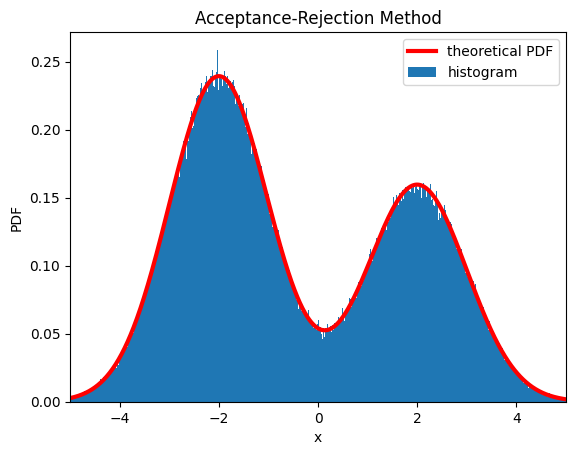
\includegraphics[width=0.5\textwidth]{./figure/p11/accept_reject.png}
\end{figure}

(d) 1. Metropolis-Hastings Algorithm: \\
Advantages: It is highly general-purpose, could applicable to a wide variety of distributions, and it does not require the normalization constant of the target distribution. \\
Disadvantages: Samples are often requires select a suitable distribution, and requires steps to burn up.

2. Hamiltonian Monte Carlo Algorithm: \\
Advantages: Due to the conservation of energy, the acceptance rate should be $1$. But there exists numerical error, however quite close to $1$, which means it has quite high acceptance rate. The samples are efficient, especially in high-dimensional problems. \\
Disadvantages: Requires computation of gradients, increasing implementation complexity. Sensitive to parameters: step size $\delta$ and number of steps for LeapFrog $L$.

3. Acceptance-Rejection Method: \\
Advantages: It produces independent samples, and is simple to implement. If the good envelope function is suitable, it is efficient. \\
Disadvantages: Efficiency depends heavily on the choice of proposal distribution, for example, ours implement has a not very high acceptance rate, which is 0.760735, but it is somehow acceptable.

\end{homeworkProblem}

\newpage